\chapter{IIR滤波器的设计}
\begin{introduction}
    \item \textit{通过滤波器设计工具生成IIR滤波器系数;}
    \item \textit{使用MATLAB仿真IIR滤波器特性;}
    \item \textit{基于FPGA实现IIR滤波器并验证其功能;}
    \item \textit{分析设计的资源消耗与时序余量。}
    \item \textit{设计流程加速方法简述}
\end{introduction}

\section{实验背景与目的}
在数字信号处理领域,FIR滤波器的设计和实现是一个重要的研究方向。相比于手动设计滤波器,使用FPGA厂商提供的IP核可以大幅简化设计流程,并提高设计的可靠性和效率。本实验旨在通过Xilinx FIR Compiler IP核实现一个FIR滤波器,研究其实现过程,并分析其资源消耗和性能。

\section{实验原理}
\subsection{FIR Compiler IP核简介}
Xilinx FIR Compiler IP核是一个高效的FIR滤波器实现工具,支持多种滤波器结构(如直接型、对称型等)和优化选项(如资源优化、性能优化)。通过该IP核,可以快速生成满足设计需求的FIR滤波器。

\subsection{设计流程}
使用FIR Compiler IP核设计FIR滤波器的基本流程如下:
\begin{enumerate}
    \item \textbf{确定滤波器参数:} 使用MATLAB或其他工具生成滤波器系数;
    \item \textbf{配置IP核:} 在Vivado中添加FIR Compiler IP核,并根据设计需求配置其参数;
    \item \textbf{生成IP核:} 生成IP核并集成到设计中;
    \item \textbf{验证功能:} 通过仿真和硬件测试验证滤波器的功能和性能。
\end{enumerate}
\section{实验使用软件/平台}
\begin{itemize}
    \item Xilinx Vivado 2024.2;
    \item eNodeX 30B软件无线电创新平台;
    \item 示波器。
    \item MATLAB \& Simulink R2024b;
  \end{itemize}
\section{实验内容}
\subsection{滤波器系数生成}
使用MATLAB的\texttt{Filter Designer}工具生成低通滤波器的系数,具体配置如下:
\begin{itemize}
    \item 滤波器类型:低通滤波器;
    \item 通带边界:800kHz;
    \item 阻带边界:3.2MHz;
    \item 采样频率:20MHz;
    \item 量化:12位定点数,1位整数部分,11位小数部分。
\end{itemize}

图~\ref{fig:filter_coefficients}展示了生成的FIR滤波器的幅频和相频特性。可以看到,滤波器在800kHz以下的频率范围内具有良好的通带特性,而在3.2MHz以上的频率范围内则具有较好的阻带特性。量化前后幅频、相频特性均变化较小,不影响性能。
\begin{figure}[htbp]
    \centering
    \includegraphics[width=0.8\textwidth]{figure/exp7/filterDesign.png}
    \caption{FIR滤波器参考/量化后幅频、相频特性}
    \label{fig:filter_coefficients}
\end{figure}

生成的滤波器系数导出为文本文件,用于配置FIR Compiler IP核。

\subsection{FIR Compiler IP核配置}
在Vivado中添加FIR Compiler IP核,并根据以下参数进行配置:
\begin{itemize}
    \item 滤波器结构:对称型;
    \item 系数输入方式:从文件导入,文件为MATLAB滤波器设计工具生成的\texttt{coe}文件;
    \item 数据位宽:输入12位有符号数,输出24位有符号数;
    \item 系数位宽:12位定点有符号数;
    \item 时钟、采样频率:20MHz(仿真时使用50MHz)。
\end{itemize}
\subsection{基于IP核的FIR滤波器设计}
仅需例化FIR Compiler IP核生成的模块即可,设计代码如代码~\ref{lst:fir_ip_ex}:
\begin{lstlisting}[language=verilog,caption={基于IP核的FIR滤波器设计},label=lst:fir_ip_ex]
    `timescale 1ns / 1ps
module fir_ip_ex (
           input                rst,  // Posedge
           input                clk,  // 20MHz
           input  signed [11:0] Xin,
           output signed [23:0] Yout
       );  //滤波后的输出数据

wire s_data_tready;
wire m_data_tvalid;
wire s_data_tvalid;
assign s_data_tvalid = !rst;

FIR fir_lp15 (
        .aclk              (clk),            // input wire aclk
        .s_axis_data_tvalid(s_data_tvalid),  // input wire s_axis_data_tvalid
        .s_axis_data_tready(s_data_tready),  // output wire s_axis_data_tready
        .s_axis_data_tdata (Xin),            // input wire [15 : 0] s_axis_data_tdata
        .m_axis_data_tvalid(m_data_tvalid),  // output wire m_axis_data_tvalid
        .m_axis_data_tdata (Yout)            // output wire [23 : 0] m_axis_data_tdata
    );



endmodule
\end{lstlisting}
\subsection{仿真测试}
Testbench代码如代码~\ref{lst:fir_ip_tb}所示,使用Vivado的仿真工具进行功能验证。采用\textit{Clock Wizard}产生50MHz仿真时钟,输入激励分别为:
\begin{itemize}
    \item 1MHz和10MHz的正弦波叠加信号;
    \item 白噪声信号。
\end{itemize}

输入激励信号由MATLAB生成,代码如下。
\begin{lstlisting}
    [language=matlab,caption={MATLAB生成激励代码},label=lst:fir_ip_tb_matlab]
    %sim_data_gen.m
    clc;
    clear 
    f1=1e6;       %信号1频率1MHz
    f2=10e6;     %信号2频率10MHz
    Fs=50e6;      %采样频率50MHz
    N=12;               %量化位数
    data_len = 2000; %生成数据长度
    
    %产生频率叠加信号
    t=0:1/Fs:(data_len-1)/Fs;
    c1=2*pi*f1*t;
    c2=2*pi*f2*t;
    s=sin(c1)+sin(c2);       
    
    %产生白噪声信号
    noise=randn(1,length(t));%产生高斯白噪声数据
    
    %归一化处理
    noise=noise/max(abs(noise));
    s=s/max(abs(s));
    
    %N位量化处理
    Q_noise=round(noise*(2^(N-1)-1));
    Q_s=round(s*(2^(N-1)-1));
    
    %绘制产生数据的时域图
    figure(1)
    subplot(211)
    plot(t(1:300),Q_s(1:300));
    xlabel('时间(s)');ylabel('幅度(v)');
    legend ('频率叠加信号');
    grid on;
    
    subplot(212)
    plot(t(1:200),Q_noise(1:200));
    xlabel('时间(s)');ylabel('幅度(v)');
    legend('白噪声信号');
    grid on;
    
    
    %求输入信号的频谱响应
    f_s=abs(fft(Q_s,1024));
    f_s=20*log10(f_s);
    f_noise=abs(fft(Q_noise));
    f_noise=20*log10(f_noise);
    
    f_s=f_s-max(f_s);
    f_noise=f_noise-max(f_noise);
    
    
    figure(2)
    subplot(211)
    L=length(f_s);
    %横坐标单位设置为MHz
    xf=0:L-1;
    xf=xf*Fs/L/10^6;     
    plot(xf(1:L/2),f_s(1:L/2));
    xlabel('频率(MHz)');ylabel('幅度(dB)');
    legend('频率叠加信号信号');
    grid on;
    
    subplot(212)
    plot(xf(1:L/2),f_noise(1:L/2));
    xlabel('频率(MHz)');ylabel('幅度(dB)');
    legend('白噪声信号');
    grid on;
    
    fid=fopen('./Bin_noise12.txt','w');
    for i=1:length(Q_noise)
        B_noise=dec2bin(Q_noise(i)+(Q_noise(i)<0)*2^N,N);
        for j=1:N
           if B_noise(j)=='1'
               tb=1;
           else
               tb=0;
           end
           fprintf(fid,'%d',tb);  
        end
        fprintf(fid,'\r\n');
    end
    fprintf(fid,';'); 
    fclose(fid);
    
    fid=fopen('./Bin_sin12.txt','w');
    for i=1:length(Q_s)
        B_s=dec2bin(Q_s(i)+(Q_s(i)<0)*2^N,N);
        for j=1:N
           if B_s(j)=='1'
               tb=1;
           else
               tb=0;
           end
           fprintf(fid,'%d',tb);  
        end
        fprintf(fid,'\r\n');
    end
    fprintf(fid,';'); 
    fclose(fid);
    \end{lstlisting}
输出为经过FIR滤波器处理后的信号。
\begin{lstlisting}[language=verilog,caption={FIR滤波器的Testbench},label=lst:fir_ip_tb]
`timescale 1ns / 1ps

module tb_FIR;
    
      // Inputs
      reg rst;
      wire clk;
      wire clk_20M;
      reg clk_100M;
      wire signed [11:0] Xin;
      wire signed [13:0] Xin_DAC;  // 14 bits signed
      // Outputs
    
      wire signed [23:0] Yout;
    
      initial begin
        // Initialize Inputs
        rst = 1;
        clk_100M = 0;
    
    
        // Wait 100 ns for global reset to finish
        #100;
        rst = 0;
        // Add stimulus here
    
      end
      always #5 clk_100M = ~clk_100M;  // 100MHz
    
      clk20m inst_clk20m (
          // Clock out ports
          .clk_out_20m(clk_20M),  // output clk_out_20M
          .clk_out_50m(clk),  // output clk_out_50M
          // Status and control signals
          .locked     (),     // output locked
          // Clock in ports
          .clk_in1    (clk)   // input clk_in1
      );
    
    
    
      INPUT_GENERATOR #(
          .CTRL_WORD_P(16'h51E),  // 1M
          .CTRL_WORD_Q(16'h28F5)  // 8M
      ) input_gen (
          .i_clk(clk),
          .o_sin_add(Xin),
          .o_sin_add_DAC(Xin_DAC)
      );
    
      fir_ip_ex sim (
          .rst (rst),
          .clk (clk),  //系统时钟50MHz
          .Xin (Xin),  //输入数据
          .Yout(Yout)  //输出数据
      );
    
      //从外部i文件读入数据作为测试激励
      //   integer i = 0;
      //   parameter sim_len = 2000;
      //   reg [11:0] sim_data[1:sim_len];
      //   always @(posedge clk) begin
      //     $readmemb("/home/liptp/ex_7/ex_7.srcs/sources_1/new/Bin_sin12.txt", sim_data);
      //     //    $readmemb("./Bin_noise12.txt",sim_data);
      //     i   = i + 1;
      //     Xin = sim_data[i];
      //   end
    
      //将仿真数据dout写入外部TXT文件中
      integer file_out;
      initial begin
    
        file_out = $fopen("/home/liptp/ex_7/ex_7.srcs/sim_1/new/sin_filter_out.txt");
        //file_out = $fopen("D:/dsp_lab_data/noise_filter_out.txt");
        if (!file_out) begin
          $display("could not open file!");
          $finish;
        end
      end
    
      //将输出数据写入指定文本文件中
      wire rst_write;
    
      //产生写入时钟信号,复位状态时不写入数据
      assign rst_write = clk & (!rst);
      always @(posedge rst_write) $fdisplay(file_out, "%d", Yout);
    
endmodule    
\end{lstlisting}

波形仿真结果(图~\ref{fig:exp7:sim_result}~)表明,滤波器能够有效滤除两种信号中的高频分量,保留低频分量。

\begin{figure}[htbp]
    \centering
    \subfloat[正弦叠加信号]{\includegraphics[width=0.45\textwidth]{figure/exp7/sim_sine.png}}
    \hfill
    \subfloat[白噪声信号]{\includegraphics[width = 0.45\textwidth]{figure/exp7/sim_noise.png}}
    \caption{仿真结果} 
    \label{fig:exp7:sim_result}   
\end{figure}

将仿真文件输出的结果写入文本文件中,使用MATLAB进行后续分析。MATLAB代码如下(代码~\ref{lst:fir_ip_tb_matlab}~),绘制了经过滤波器处理后的信号的幅频响应曲线。可以看到,经过滤波器处理后,信号的高频分量被有效滤除,保留了低频分量。
\begin{lstlisting}[language=matlab,caption={MATLAB结果绘图代码},label=lst:fir_ip_tb_matlab]
%sim_data_Analyse.m
%采样频率为50MHz
clear;
Fs=50e6;        
%从文本文件中读取数据
fid=fopen('./sin_filter_out.txt','r');
%fid=fopen('D:\dsp_lab_data\noise_filter_out.txt','r');
[dout,count]=fscanf(fid,'%lg',inf);
fclose(fid);

%求信号的幅频响应
f_out=20*log10(abs(fft(dout,1024)));
f_out=f_out-max(f_out);

%设置幅频响应的横坐标单位为MHz
x_f=[0:(Fs/length(f_out)):Fs/2]/10^6;
%只显示正频率部分的幅频响应
mf_noise=f_out(1:length(x_f));

%绘制幅频响应曲线
plot(x_f,mf_noise);
xlabel('频率(MHz)');ylabel('幅度(dB)');
grid on;

\end{lstlisting}

\begin{figure}[htbp]
    \centering
    \subfloat[频率叠加与白噪声信号输入时域波形]{\includegraphics[width=0.45\textwidth]{figure/exp7/mat_1.png}}
    \hfill
    \subfloat[频率叠加与白噪声信号输入频谱]{\includegraphics[width=0.45\textwidth]{figure/exp7/mat_2.png}}
    \\
    \subfloat[频率叠加信号滤波输出频谱]{\includegraphics[width=0.45\textwidth]{figure/exp7/mat_3.png}}
    \hfill
    \subfloat[白噪声信号滤波输出频谱]{\includegraphics[width=0.45\textwidth]{figure/exp7/mat_4.png}}
    \caption{MATLAB分析的输入信号与滤波结果}
    \label{fig:exp7:matlab_results}
\end{figure}
\subsection{硬件实现与验证}
将生成的FIR Compiler IP核集成到设计中,连接板载输入输出信号,并通过ILA波形和示波器波形验证滤波器的功能。测试输入信号为叠加的250kHz和4MHz正弦波,测试时钟为20MHz,验证滤波器是否能够有效滤除4MHz分量。

顶层模块代码如下:
\begin{lstlisting}[language=verilog,caption={顶层模块代码},label=lst:top_module]
`timescale 1ns / 1ps
module top_mod (
               // DAC PINS
               output signed [13:0] LS_DAC2_DB,
               output LS_DAC2_CLK,
               output LS_DAC2_WRT,
               output signed [13:0] LS_DAC1_DB,
               output LS_DAC1_CLK,
               output LS_DAC1_WRT,
    
               output LS_DAC_MODE,
    
    
               // ADC PINS
               input [11:0] LS_ADC2_DB,
               input [11:0] LS_ADC1_DB,
               input LS_ADC2_OTR,
               input LS_ADC1_OTR,
               output LS_ADC2_CLK,
               output LS_ADC1_CLK,
    
               // GPIOs IO PINs
               // output GPIO_TH1, GPIO_TH2, GPIO_TH3, GPIO_TH4, GPIO_TH5,
               // output GPIO_TH6, GPIO_TH7, GPIO_TH8, GPIO_TH9, GPIO_TH10
    
               input PL_CLK_100MHz  // Clk 100MHz
           );
    
    wire clk_20M;
    wire clk_locked;
    wire signed [11:0] xin;
    wire signed [25:0] yout;
    wire signed [13:0] xin_DAC;
    reg signed [11:0] xin_ADC;
    
    
    always @(posedge clk_20M) begin
        xin_ADC <= LS_ADC1_DB;
    end
    
    clk20m inst_clk20m (
               // Clock out ports
               .clk_out_20m(clk_20M),       // output clk_out_20M
               .clk_out_6_25(),             // output 6.25MHz, we don't use it
               // Status and control signals
               .locked     (),              // output locked
               // Clock in ports
               .clk_in1    (PL_CLK_100MHz)  // input clk_in1
           );
    
    
    ila_0 inst_ila (
              .clk(clk_20M),  // input wire clk
              .probe0(LS_DAC1_DB),  // input wire [13:0]  probe0 ,
              .probe1(LS_DAC2_DB)  // input wire [13:0]  probe1
          );
    
    fir_ip_ex fir (
                  .rst (1'b0),  // Posedge
                  .clk (clk_20M),   // 20MHz
                  .Xin (xin_ADC),
                  .Yout(yout)
              );
    
    INPUT_GENERATOR #(
                        .CTRL_WORD_P(16'h199),  // 0.25M
                        .CTRL_WORD_Q(16'h1999)  // 4M
                    ) input_gen (
                        .i_clk(clk_20M),
                        .o_sin_add(xin),
                        .o_sin_add_DAC(xin_DAC)
                    );
    
    
    // DAC OUTPUT
    assign LS_DAC_MODE = 1'b1;
    assign LS_DAC1_DB  = xin_DAC + 14'h2000;
    assign LS_DAC1_CLK = !clk_20M;
    assign LS_DAC1_WRT = LS_DAC1_CLK;
    assign LS_DAC2_DB  = yout[25:12] + 14'h2000;
    assign LS_DAC2_CLK = clk_20M;
    assign LS_DAC2_WRT = LS_DAC2_CLK;
    
    // ADC Clock Dump
    
    assign LS_ADC1_CLK = clk_20M;
    
endmodule
\end{lstlisting}    

如图~\ref{fig:exp7:waveform},将eNodeX 1口接入示波器,可观察到叠加频率的输入信号(未经ADC采样);将ADC端口接入1口,2口接示波器,可获得ADC以20MHz采样频率采样的输入信号经过滤波后的输出结果。
\begin{figure}[htbp]
  \centering
  \subfloat[输入信号]{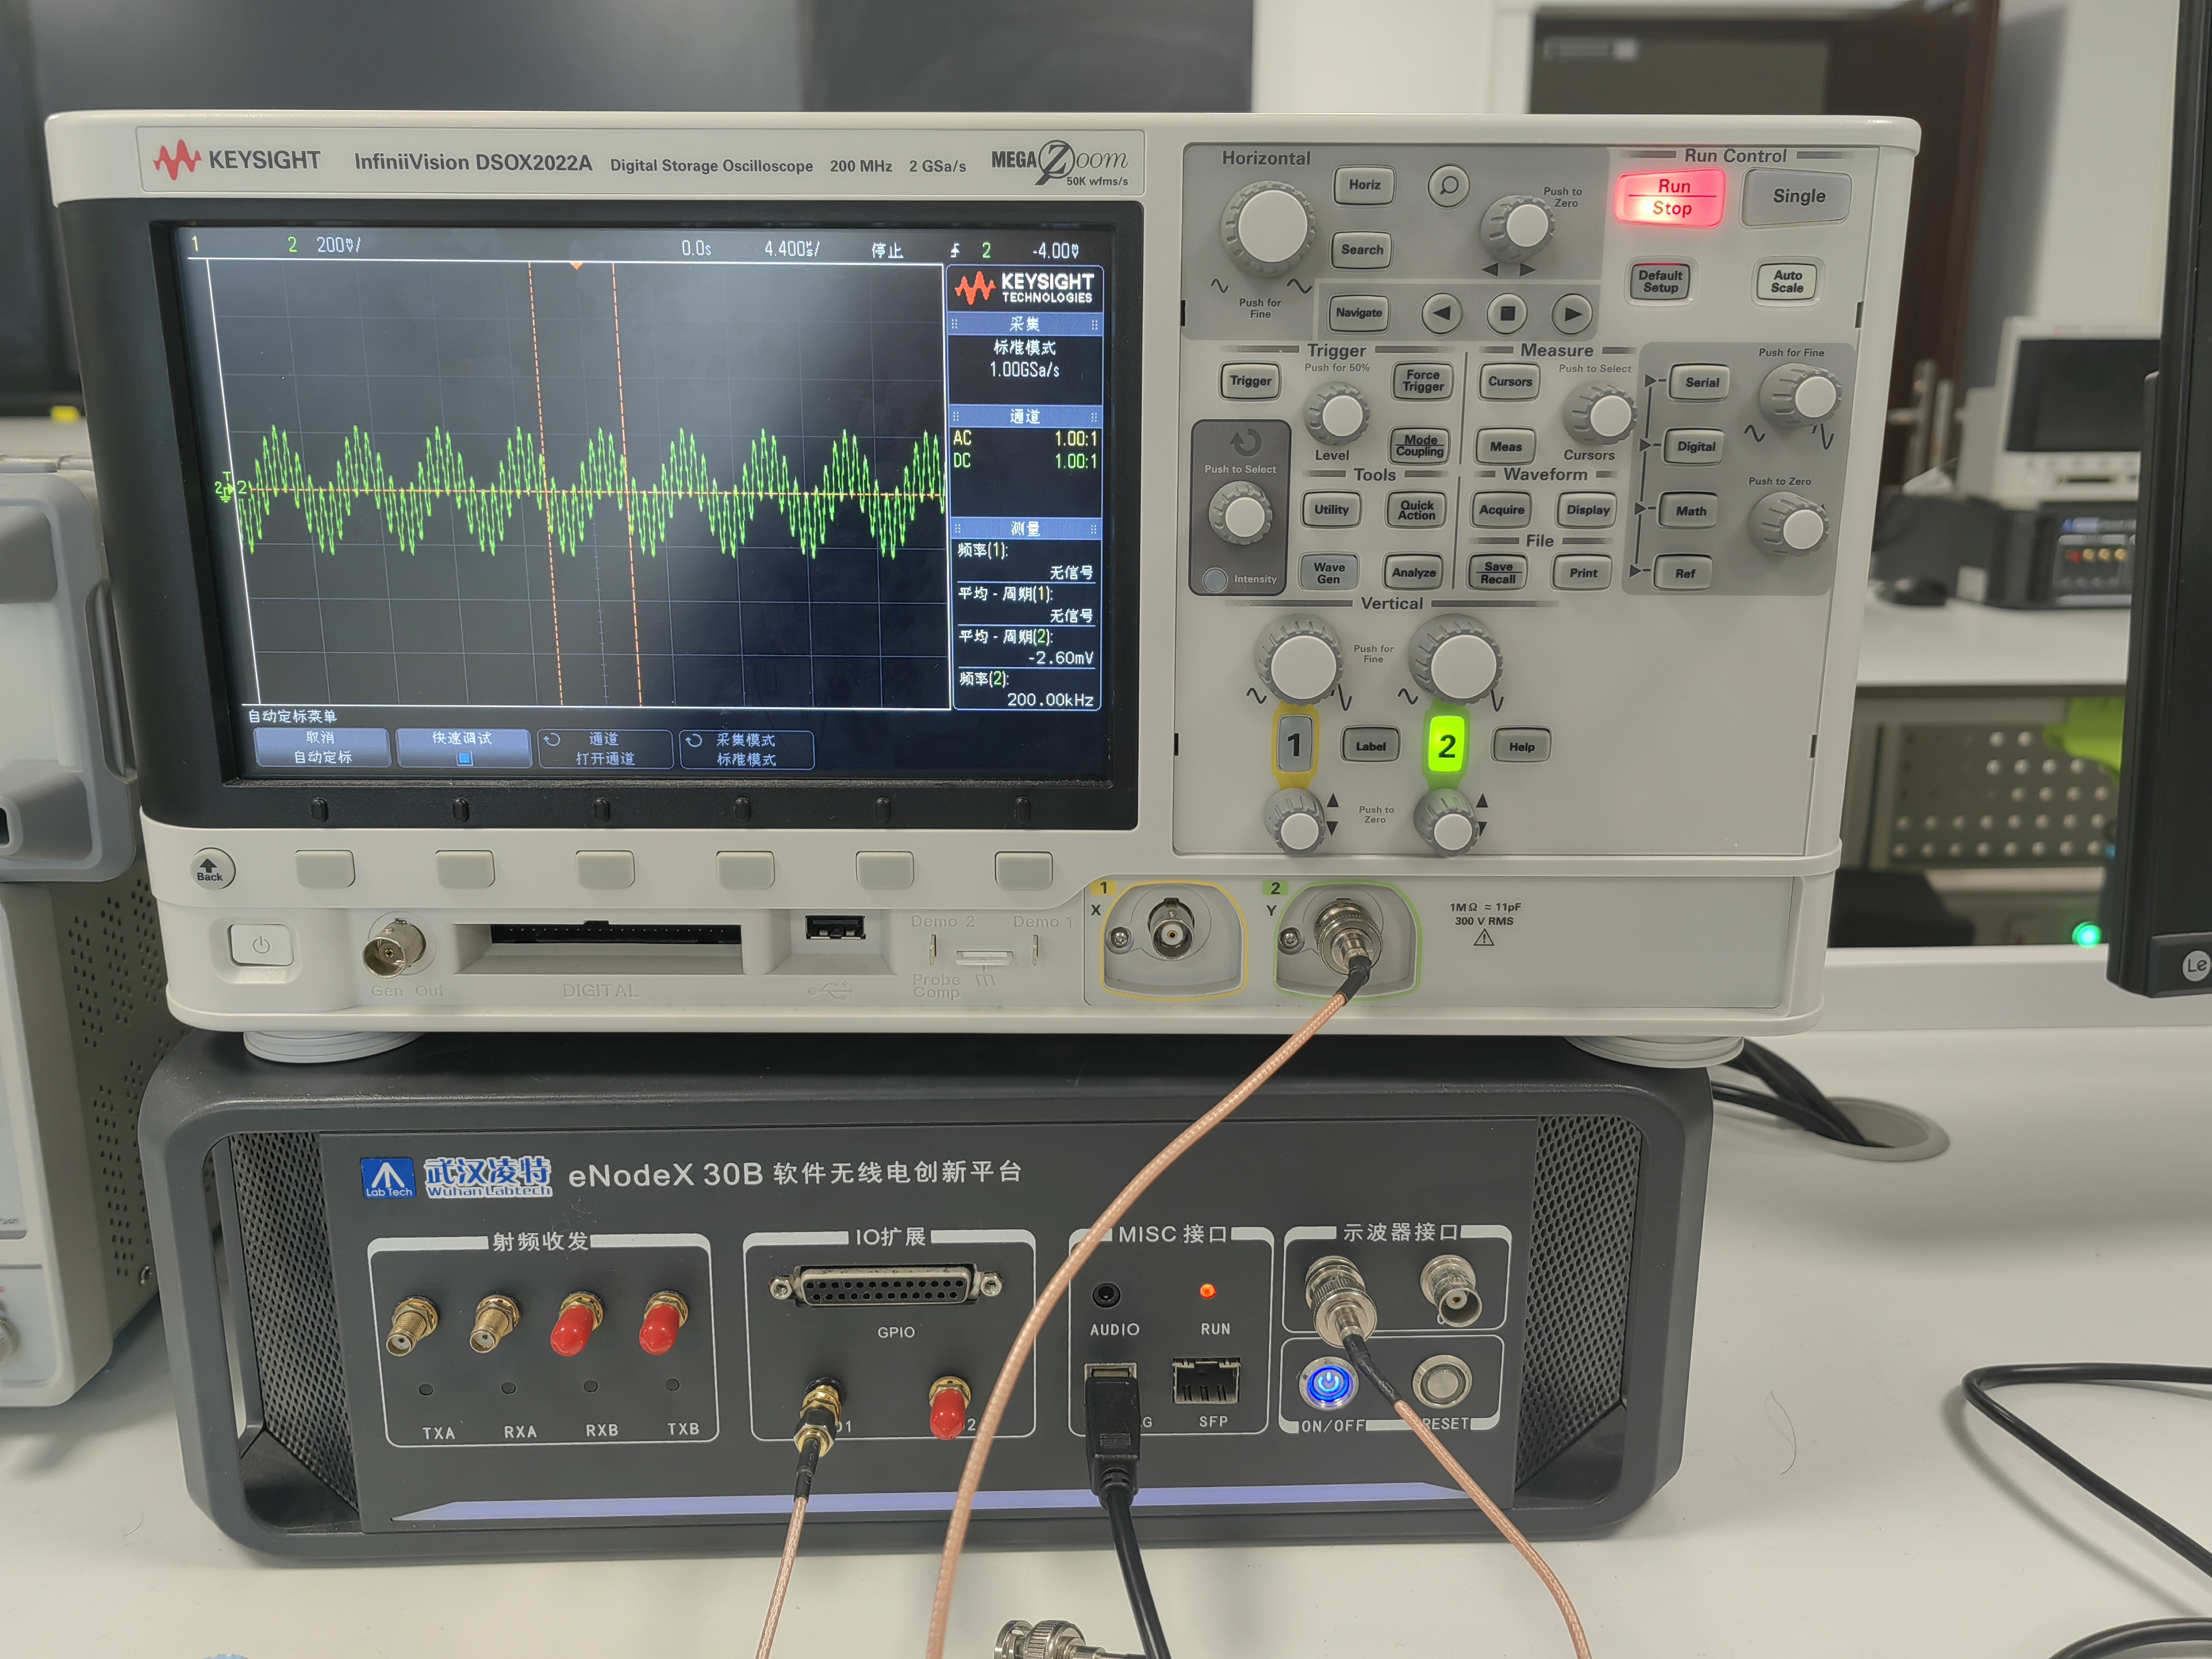
\includegraphics[width=0.35\textwidth]{figure/exp7/input_7.jpg}}
    \hspace{0.05\textwidth}
  \subfloat[输出信号]{\includegraphics[width=0.35\textwidth]{figure/exp7/output_7.jpg}}
  \caption{FIR滤波器输入输出信号的示波器波形}
  \label{fig:exp7:waveform}
\end{figure}

打开硬件波形查看器ILA,可观察到输出波形中滤除了输入波形中的高频分量。(图~\ref{fig:exp7:sim:ILA})
\begin{figure}[htbp]
  \centering
  \includegraphics[width = 0.95\textwidth]{figure/exp7/ILA.png}
  \caption{ILA波形}
  \label{fig:exp7:sim:ILA}
\end{figure}

\subsection{资源消耗分析}
Vivado的资源报告如图~\ref{fig:exp7:resource_analysis}所示(包含TOP模块),展示了使用FIR Compiler IP核实现的滤波器在FPGA上的资源消耗情况。可以看到,设计使用了较少的LUT和FF资源,同时DSP资源的使用也在合理范围内。注意到FIR滤波器会使用MMCM资源,因此在实际使用时要合理分配FPGA资源。

\begin{figure}[htbp]
    \centering
    \includegraphics[width=0.45\textwidth]{figure/exp7/util_summary.png}
    \caption{资源消耗分析}
    \label{fig:exp7:resource_analysis}
\end{figure}
\subsection{时序分析}

时序分析表明,设计满足50MHz的时钟频率要求。
\begin{figure}[htbp]
    \centering
    \includegraphics[width=0.8\textwidth]{figure/exp7/timing_summary.png}
    \caption{时序分析结果}
    \label{fig:exp7:time_analysis}
\end{figure}

具体分析:

\textbf{Setup:}  
\begin{itemize}
  \item Worst Negative Slack (WNS): 26.691 ns。表示最差的负时序余量,值为26.691纳秒,说明在时序上存在一定的余量,设计没有违反时序约束。  
\item Total Negative Slack (TNS): 0.00 ns。表示总的负时序余量为零,说明所有时序约束都被满足。  
\item Number of Failing Endpoints: 0。表示没有时序失败的端点,所有的时序约束都符合要求。  
\item Total Number of Endpoints: 5364。表示在设计中,共有5364个时序端点。
\end{itemize}


\textbf{Hold:}  
\begin{itemize}
\item Worst Hold Slack (WHS): 0.300 ns。表示最差的保持时序余量,值为0.300纳秒,表明该设计在保持时序方面没有违反约束。  
\item Total Hold Slack (THS): 0.00 ns。表示总的保持时序余量为零,表明所有保持时序约束都被满足。  
\item Number of Failing Endpoints: 0。表示没有违反保持时序约束的端点。  
\item Total Number of Endpoints: 5348。表示共有5348个端点。
\end{itemize}

\textbf{Pulse Width:}  
\begin{itemize}
  \item Worst Pulse Width Slack (WPWS): 9.500 ns。表示最差的脉冲宽度时序余量,值为9.500纳秒,说明设计在脉冲宽度方面有足够的时序余量。  
  \item Total Pulse Width Negative Slack (TPWS): 0.00 ns。表示总的脉冲宽度负时序余量为零,表明所有脉冲宽度时序约束都得到满足。  
  \item Number of Failing Endpoints: 0。表示没有违反脉冲宽度时序约束的端点。  
\item Total Number of Endpoints: 284。表示共有2688个端点。
\end{itemize}

可以看到 WNS 远远大于之前代码实现的 FIR 滤波器,故从时序余量上看, IP 核实现 的滤波器性能优于代码实现的滤波器。
\section{思考与讨论}
\subsection{IP核设计的优缺点}
\begin{itemize}
    \item 与手动设计的滤波器相比,使用IP核的设计流程更加高效,但灵活性较低;
    \item IP核的资源消耗和性能表现与配置参数密切相关,需要根据具体需求进行权衡;
    \item 在实际应用中,可以结合手动设计和IP核的优点,选择最优的实现方式。
\end{itemize}
\subsection{基于IP核的半串行结构的FIR滤波器}

添加一个二分频器,用作IP核的使能信号,设计代码如代码~\ref{lst:fir_ip_ex2}所示。可以看到,IP核的使能信号为二分频器的输出信号。
\begin{lstlisting}[language=verilog,caption={基于IP核的半串行结构的FIR滤波器},label=lst:fir_ip_ex2]
module fir_ip_ex(
input rst, //复位信号,高电平有效
input clk, //FPGA 系统时钟,频率为 50MHz
input signed [11:0] Xin, //输入数据
output signed [23:0] Yout //滤波后的输出数据
);
wire s_data_tready;
wire m_data_tvalid;
reg [11:0] Xin_reg;
reg s_data_tvalid;
reg toggle; // 用来实现二分频采样
// 二分频逻辑
always @(posedge clk or posedge rst) begin
if (rst) begin
toggle <= 1'b0;
end else begin
toggle <= ~toggle; // 每个 50M 时钟翻转一次,得到 25M 使能
end
end
// 控制 tvalid 和输入数据
always @(posedge clk or posedge rst) begin
if (rst) begin
Xin_reg <= 12'd0;
s_data_tvalid <= 1'b0;
end else begin
if (toggle) begin
Xin_reg <= Xin;
s_data_tvalid <= 1'b1; // 只有在 toggle 为 1 时才发送数据
end else begin
s_data_tvalid <= 1'b0; // toggle 为 0 时不发送
end
end
end
// 实例化 FIR IP
fir_compiler_0 fir_lp15 (
.aclk(clk), // input wire aclk
.s_axis_data_tvalid(s_data_tvalid), // input wire s_axis_data_tvalid
.s_axis_data_tready(s_data_tready), // output wire s_axis_data_tready
.s_axis_data_tdata(Xin_reg), // input wire [15 : 0] s_axis_data_tdata
.m_axis_data_tvalid(m_data_tvalid), // output wire m_axis_data_tvalid
 .m_axis_data_tdata(Yout) // output wire [23 : 0] m_axis_data_tdata
);
endmodule
\end{lstlisting}

得到仿真结果如图~\ref{fig:exp7:sim_result2}~所示:
\begin{figure}[htbp]
    \centering
    \subfloat[正弦叠加信号]{\includegraphics[width=0.45\textwidth]{figure/exp7/sin_half_serial.png}}
    \hfill
    \subfloat[白噪声信号]{\includegraphics[width = 0.45\textwidth]{figure/exp7/noise_half_serial.png}}
    \caption{仿真结果} 
    \label{fig:exp7:sim_result2}
\end{figure}

\section{实验流程加速框架简述}
在《系统实验》这门课这次以及之前的实验中,可以发现一次完整的信号分析流程大抵相同,主要包括以下几个步骤:
\begin{itemize}
    \item 通过FFT IP核的功能仿真确定待滤波信号频谱(实验需求);
    \item 指定滤波器类型,输入信号频率,采样频率等;
    \item 使用高级语言,如MATLAB的\texttt{Filter Designer}工具生成滤波器系数,验证幅频响应,并导出COE系数文件用作滤波器系数;
    \item 编写RTL代码或调用IP核,实现滤波器的硬件设计;
    \item 编写测试Testbench,进行功能仿真验证,并验证时序是否违例,生成资源消耗情况报告;
    \item 使用ADC或DDS输入数据,例化相应IP核,并设置ILA观测信号接口。
    \item 写比特流验证,通过配套硬件接口,如eNodeX 30B软件无线电创新平台进行硬件验证。在此过程中通过ILA观察输入输出信号的波形。
\end{itemize}

传统的实验方式需要每次从MATLAB GUI中手动导出COE文件,并在Vivado FIR IP核中引用该COE文件。并且,现有的设计流程需要每次在RTL设计中修改输入输出位宽,并手动修改FIR和FFT IP核的配置参数,过程繁杂且易出错,无法满足快速参数化设计的需求。为此,我们提出一种基于python \texttt{matplotlib, scipy, verithon} 库和Vivado tcl脚本的设计流程加速框架。目前,用户可以基于此框架完成以下功能:
\begin{itemize}
    \item 生成任意幅度、相位、长度的正弦序列,并支持信号运算、信号定点量化、信号时域/频域分析和信号导出(COE格式或TXT格式);
    \item 使用\texttt{scipy.signal}库设计滤波器,用户仅需传入滤波器类型、采样频率、通带阻带边界、滤波器阶数、量化位宽参数,即可自动生成滤波器系数和查看滤波器幅频响应,并提供导出COE格式文件的API;
    \item 提供FFT、串行、并行、半串行FIR滤波器、IIR滤波器的设计模板(基于做过的实验),用户在python层指定参数后,即可自动生成正确位宽的RTL代码。
    \item 提供\texttt{FIR compiler}, \texttt{xfft} IP核的tcl脚本,系统目前支持自动推断IP核需修改的配置参数。
    \item 提供自动生成Testbench的API(文件读写形式的测试),用户可以灵活地指定时钟、复位和输入输出形式。
\end{itemize}

目前该框架还在不断完善中,由于即将期末考试,对该项目的开发有所延缓。后续会继续完善该框架,力求实现自动化的实验流程。项目代码目前托管在Github上,地址为\url{https://github.com/LiPtP0000/system_experiment_autogen}。